
\begin{frame}{Bonnes pratiques dans le numérique}{Conseils 11-14/115}

\begin{block}{Favoriser un développement sur-mesure à l'usage d'un CMS}
Les CMS utilisent des systèmes de "hook".
\end{block}

\begin{block}{Favoriser les pages statiques}
pour une landing page ou simple site vitrine de créer un site statique en HTML, CSS et JS.
\end{block}

\begin{block}{Créer une architecture applicative modulaire}
Les logiciels open source les plus efficients, comme nginX, Apache, MySQL ou PHP, reposent sur cette architecture modulaire.

Côté backend, le découpage en microservices permet d'apporter un niveau de modularité pour des services HTTP. 
\end{block}


\begin{block}{Choisir les technologies les plus adaptées}
 Sélectionner l’outil le plus économe en fonction de ses besoins et de ses contraintes métier.
\end{block}

\end{frame}


\begin{frame}{Bonnes pratiques dans le numérique}{Conseil 15/115}

\begin{block}{Utiliser certains forks applicatifs orientés "performance"}

\begin{itemize}
    \item À Redis, préférer plutôt la version optimisée KeyDB.
    \item À Drupal, préférer plutôt la version optimisée Pressflow.
\end{itemize}
\end{block}


\begin{minipage}[b]{0.4\linewidth}  
\begin{figure}
    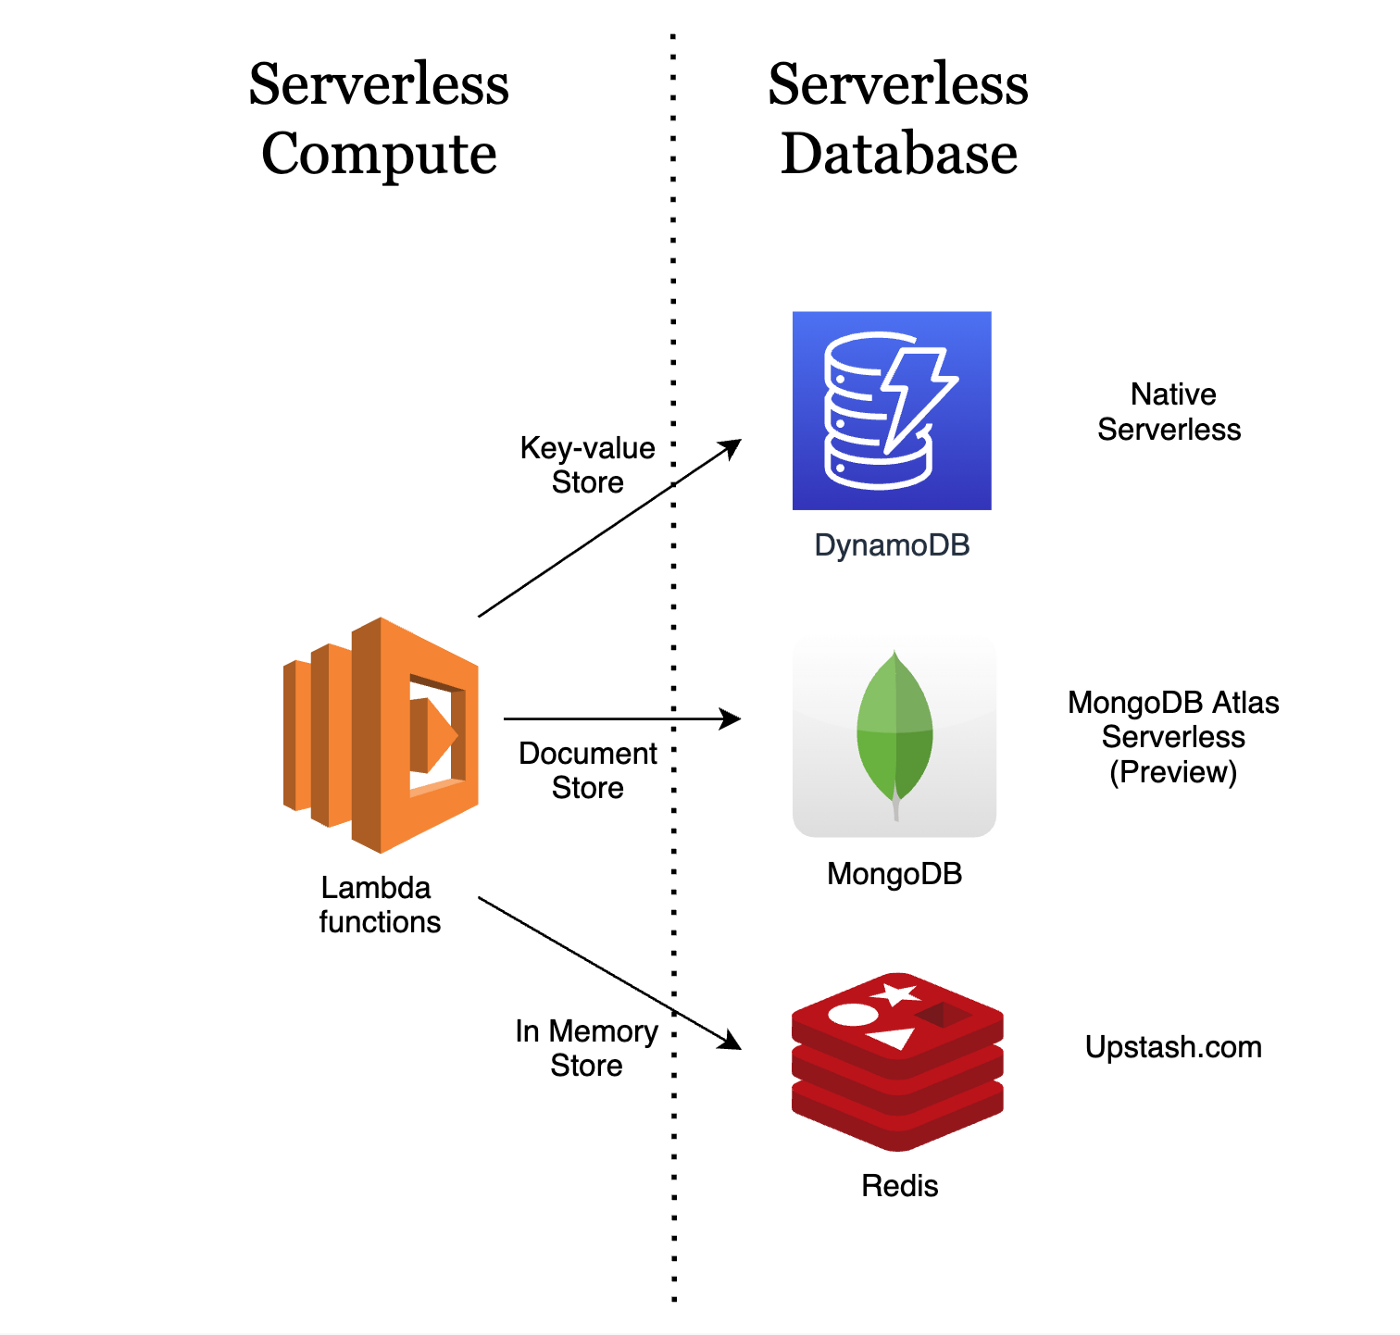
\includegraphics[scale=0.1]{chapitre2/wdd2/fig/redis.png}
    \centering
\end{figure}
\end{minipage}\hfill
\begin{minipage}[b]{0.6\linewidth}  
\begin{figure}
    \centering
    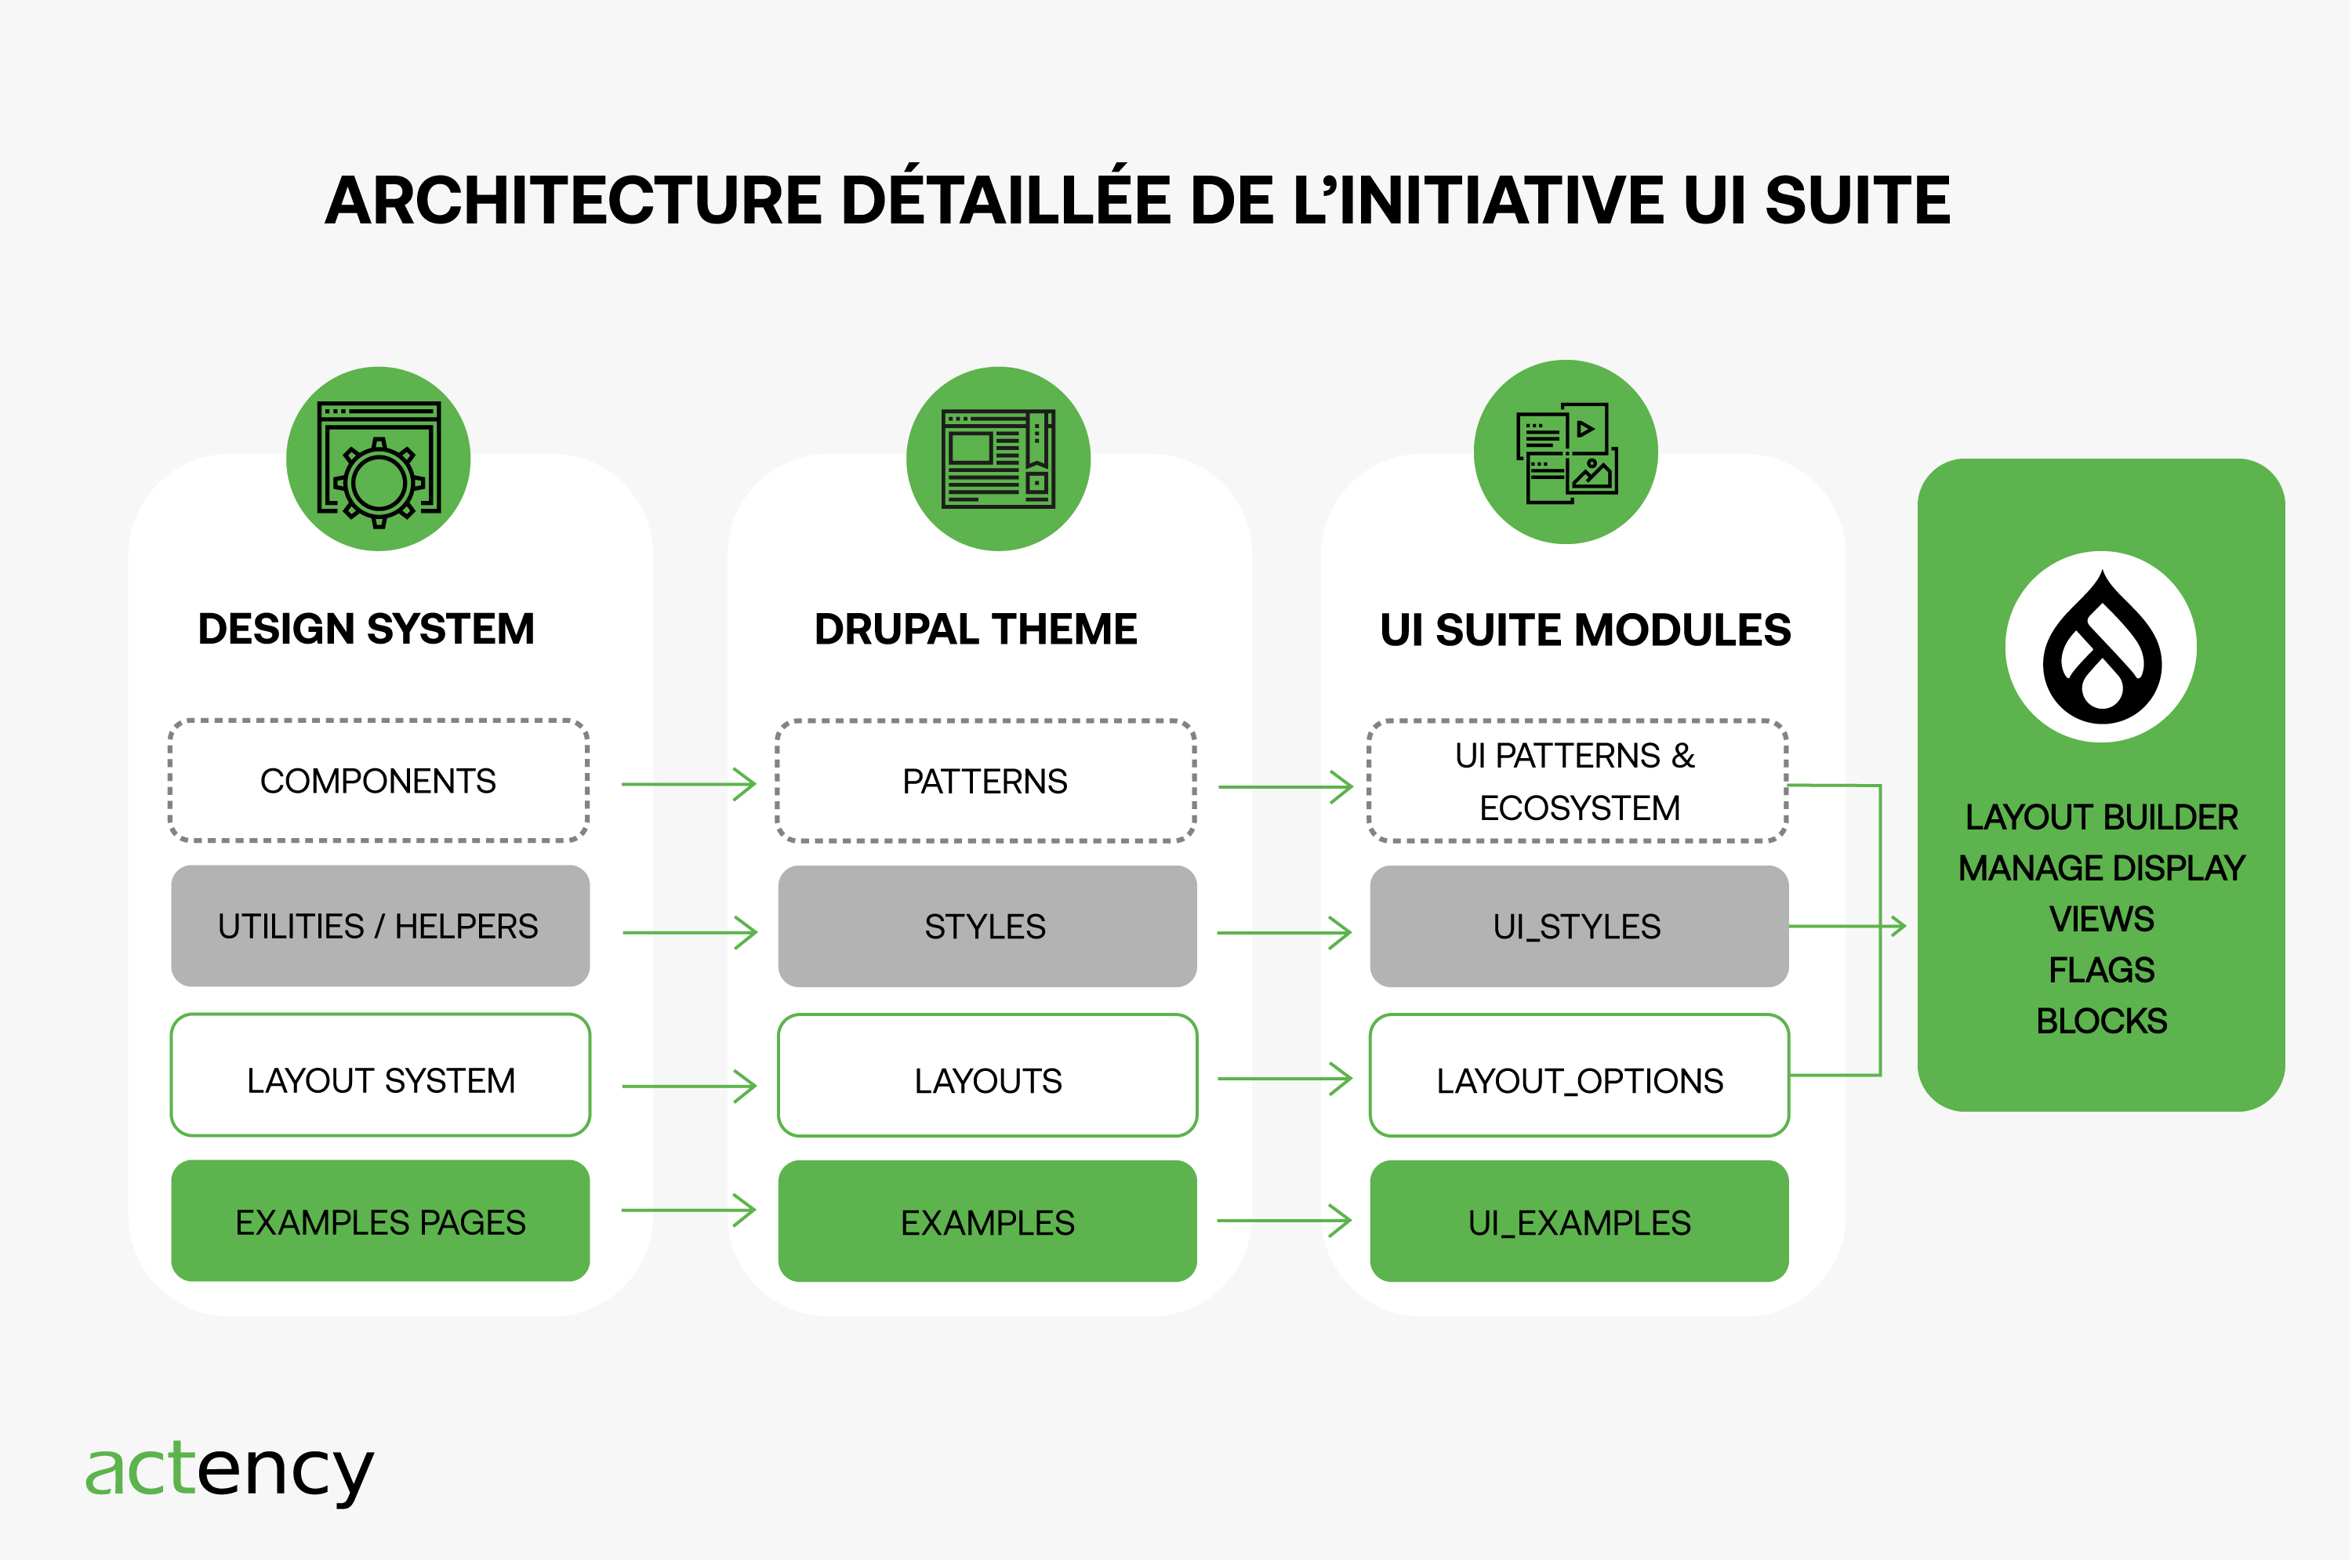
\includegraphics[scale=0.07]{chapitre2/wdd2/fig/drupal.jpg}
\end{figure}
\end{minipage}\hfill


\end{frame}

\begin{frame}{Bonnes pratiques dans le numérique}{Conseils 16-18/115}

\begin{block}{Choisir un format de données adapté}
Le type de données utilisé pour manipuler et stocker une donnée a un impact significatif sur la consommation mémoire et les cycles.
\end{block}

\begin{block}{Limiter le nombre de domaines servant les ressources}
 Regrouper toutes les ressources sur un seul domaine.
 \end{block}

\begin{block}{Remplacer les boutons officiels de partage des réseaux sociaux}
Préférer des liens HTML aux plugins JavaScript
\begin{figure}
    \centering
    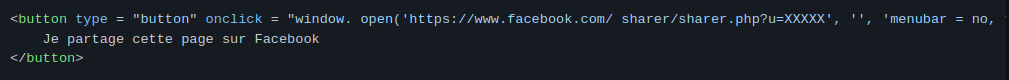
\includegraphics[scale=0.305]{chapitre2/wdd2/fig/code.png}
\end{figure}


 \end{block}
 
 
 
\end{frame}




\begin{frame}{Bonnes pratiques dans le numérique}{Conseils 19-21/115}

\begin{block}{Découper les CSS}
Employer un ensemble de CSS plutôt qu’une seule, et appeler uniquement les CSS utiles.
 \end{block}

\begin{block}{Limiter le nombre de CSS}
Limiter le nombre de CSS pour ne pas multiplier les requêtes HTTP et pour simplifier le rendu côté navigateur.

\begin{figure}
    \centering
    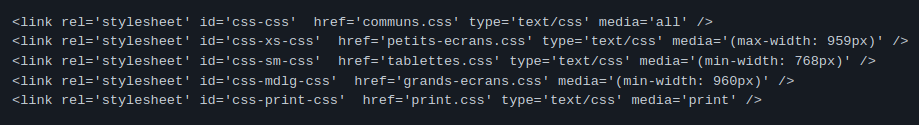
\includegraphics[scale=0.33]{chapitre2/wdd2/fig/codeL.png}
\end{figure}

 \end{block}

\begin{block}{Préférer les CSS aux images}
Utiliser les propriétés CSS3 à la place d’images. 
 \end{block}


 
\end{frame}


\begin{frame}{Pause débunkage }{Fake checking : les lampes à décharge et à led}
\begin{figure}
    \centering
    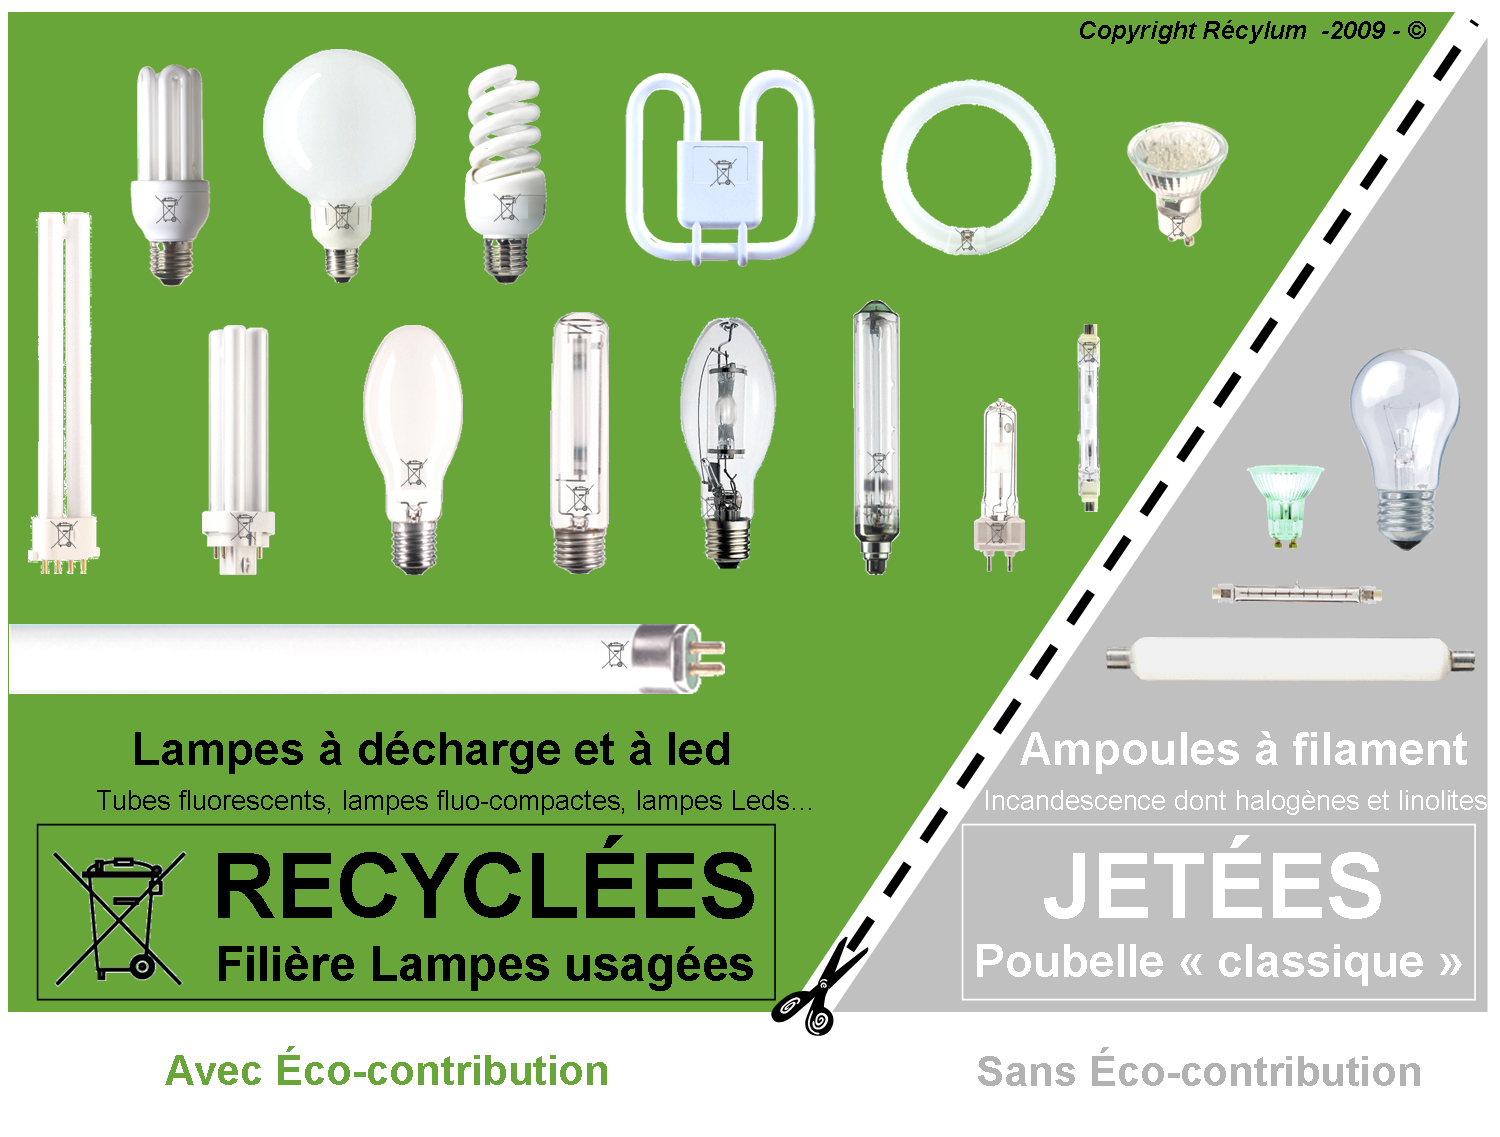
\includegraphics[scale=0.35]{chapitre2/wdd2/fig/ampoules.png}
\end{figure}

 
\end{frame}
